% networkflow.tex
% Updated January 11, 2012

\chapter{Network Flows}\label{ch:networkflow}

This chapter continues our look at the topics of algorithms and
optimization. On an intuitive level, networks and network flows are
fairly simple. We want to move something (merchandise, water, data)
from an initial point to a destination. We have a set of intermediate
points (freight terminals, valves, routers) and connections between
them (roads, pipes, cables) with each connection able to carry a
limited amount. The natural goal is to move as much as possible from
the initial point to the destination while respecting each
connection's limit. Rather than just guessing at how to perform this
maximization, we will develop an algorithm that does it. We'll also
see how to easily justify the optimality of our solution though the
classic Max Flow-Min Cut Theorem.

\section{Basic Notation and Terminology}\label{s:networkflow:intro}

Recall that a directed graph in which for each pair of vertices $x,y$
at most one of the directed edges $(x,y)$ and $(y,x)$ between them is
present is called an \emph{oriented graph}. The basic setup for a
network flow problem begins with an oriented graph $\bfG$, called a
\textit{network}, in which we have two special vertices called the
\textit{source} and the \textit{sink}.  We use the letter $S$ to
denote the source, while the letter $T$ is used to denote the sink
(terminus).  All edges incident with the source are oriented away from
the source, while all edges incident with the sink are oriented with
the sink.  Futhermore, on each edge, we have a non-negative
\textit{capacity}, which functions as a constraint on how much can be
transmitted via the edge. The capacity of the edge $e=(x,y)$ is
denoted $c(e)$ or by $c(x,y)$.  In a computer program, the nodes of a
network may be identified with integer keys, but in this text, we will
typically use letters in labeling the nodes of a network.  This helps
to distinguish nodes from capacities in diagrams of networks.  We
illustrate a network in \autoref{fig:networkflow:network}. The numbers
associated with the edges are their capacities, so, for instance,
$c(E,B)=24$ and $c(A,T)=56$.

\begin{figure}
\centering
\includegraphics*[width=2.5in]{networkflow-figs/webfig-31a}\\
\caption{A Network}\label{fig:networkflow:network}
\end{figure}

A \textit{flow} $\phi$ in a network is a function which assigns to
each directed edge $e=(x,y)$ a non-negative value
$\phi(e)=\phi(x,y)\leq c(x,y)$ so that the following ``conservation''
laws hold:

\begin{enumerate}
\item $\sum_{x} \phi(S,x)= \sum_{x} \phi(x,T)$, i.e., the amount leaving
the source is equal to the amount arriving at the sink.  This quantity
is called the \textit{value} of the flow $\phi$.
\item For every vertex $y$ which is neither the source nor the
sink, $\sum_{x}\phi(x,y)= \sum_{x}\phi(y,x)$, i.e., the amount leaving $y$ 
is equal to the amount entering $y$.
\end{enumerate}

We illustrate a flow in a network in
\autoref{fig:networkflow:netflow}. 
\begin{figure}[hb]
\begin{center}
\includegraphics*[width=2.5in]{networkflow-figs/webfig-31b}\\
\caption{A Network Flow}\label{fig:networkflow:netflow}
\end{center}
\end{figure}
In this figure, the numbers associated with each edge are its capacity
and the amount of flow that $\phi$ places on that edge. For example,
the edge $(E,D)$ has capacity $20$ and currently carries a flow of
$8$. (Since $\phi(x,y)\leq c(x,y)$, it is always easy to determine
which number is the capacity and which is the flow.) The value of this
flow is $30 = \phi(S,F)+\phi(S,B)+\phi(S,E)=\phi(A,T)+\phi(C,T)$. To
see that the second conservation law holds at, for example, vertex
$B$, note that the flow into $B$ is $\phi(S,B)+\phi(E,B)+\phi(D,B) =
20$ and the flow out of $B$ is $\phi(B,F)+\phi(B,A)+\phi(B,C)=20$.

\begin{remark}
  Given a network, it is very easy to find a flow.  We simply assign
  $\phi(e)=0$ for every edge $e$. It is very easy to
  \textit{underestimate} the importance of this observation,
  actually. Network flow problems are a special case of a more general
  class of optimization problems known as \emph{linear programs}, and
  in general, it may be very difficult to find a feasible solution to
  a linear programming problem.  In fact, conceptually, finding a
  feasible solution---\textit{any} solution---is just as hard as
  finding an \textit{optimal} solution.
\end{remark}

\section{Flows and Cuts}\label{s:networkflow:flows-cuts}

Considering the applications suggested at the beginning of the
chapter, it is natural to ask for the maximum value of a flow in a
given network. Put another way, we want to find the largest number
$v_0$ so that there exists a flow $\phi$ of value $v_0$ in the
network. Of course, we not only want to find the maximum value $v_0$,
but we also want to find a flow $\phi$ having this value.  Although it
may seem a bit surprising, we will develop an efficient algorithm
which (a)~finds a flow of maximum value, and (b)~finds a certificate
verifying the claim of optimality.  This certificate makes use of the
following important concept.

A partition $V=L\cup U$ of the vertex set $V$ of a network 
with $S\in L$ and $T\in U$ is called a
\textit{cut}.\footnote{Our choice of $L$ and $U$ for the names of the
  two parts of the partition will make more sense later in the
  chapter.}  The \textit{capacity} of a cut $V=L\cup U$, denoted
$c(L,U)$, is defined by
\[
c(L,U) = \sum_{x\in L,y\in U} c(x,y).
\]
Put another way, the capacity of the cut $V=L\cup U$ is the total
capacity of all edges \emph{from} $L$ \emph{to} $U$. Note that in
computing the capacity of the cut $V=L\cup U$, we only add the
capacities of the edges from $L$ to $U$.  We do \emph{not} include the
edges from $U$ to $L$ in this sum.

\begin{example}
  Let's again take a look at the network in
  \autoref{fig:networkflow:netflow}. Let's first consider the cut
  $V=L_1\cup U_1$ with
  \[L_1 = \{S,F,B,E,D\}\qquad\text{and}\qquad U_1= \{A,C,T\}.\]
  Here we see that the capacity of the cut is
  \[c(L_1,U_1) = c(F,A) + c(B,A) + c(B,C)+ c(D,C) = 24+15+20+42 =
  101.\]
  We must be a bit more careful, however, when we look at the cut
  $V=L_2\cup U_2$ with
  \[L_2 = \{S,F,B,E\}\qquad\text{and}\qquad U_2=\{A,D,C,T\}.\]
  Here the capacity of the cut is
  \[c(L_2,U_2) = c(F,A) + c(B,A) + c(B,C) + c(E,D) = 24+15+20+20=79.\]
  Notice that we do not include $c(D,B)$ in the calculation as the
  directed edge $(D,B)$ is from $U_2$ to $L_2$.
\end{example}

The relationship between flows and cuts rests on the following
fundamentally important theorem.

\begin{theorem}\label{thm:networkflow:flowleqcut}
Let $\GVE$ be a network, let $\phi$ be a flow in $\bfG$ and let 
$V=L\cup U$ be a cut. Then the value of the flow is at most as
large as the capacity of the cut.
\end{theorem}
\begin{proof}
  In this proof (and throughout the chapter), we adopt the very
  reasonable convention that $\phi(x,y)=0$ if $(x,y)$ is not a
  directed edge of a network $\bfG$. 

  Let $\phi$ be a flow of value $v_0$ and let $V=L\cup U$ be a
  cut. First notice that
  \[v_0 = \sum_{y\in V} \phi(S,y) - \sum_{z\in V}\phi(z,S),\]
  since the second summation is $0$. Also, by the second of our flow
  conservation laws, we have for any vertex other than the source and
  the sink,
  \[\sum_{y\in V}\phi(x,y) -\sum_{z\in V}\phi(z,x) = 0.\]
  Now we have
  \begin{align*}
    v_0 &= \sum_{y\in V} \phi(S,y) - \sum_{z\in V}\phi(z,S)\\
    &= \sum_{y\in V} \phi(S,y) - \sum_{z\in V}\phi(z,S) +
    \sum_{\substack{x\in L\\x\neq S}}\left[\sum_{y\in V} \phi(x,y) -
      \sum_{z\in V}\phi(z,x)\right]\\
    &= \sum_{x\in L}\left[\sum_{y\in V} \phi(x,y) -
      \sum_{z\in V}\phi(z,x)\right]
  \end{align*}
  At this point, we want to pause and look at the last line. Notice
  that if $(a,b)$ is a directed edge with both endpoints in $L$, then
  when the outer sum is conducted for $x=a$, we get an overall
  contribution of $\phi(a,b)$. On the other hand, when it is conducted
  for $x=b$, we get a contribution of $-\phi(a,b)$. Thus, the terms
  cancel out and everything simplifies to
  \[\sum_{\substack{x\in L\\y\in U}} \phi(x,y) - \sum_{\substack{x\in
      L\\ z\in U}} \phi(z,x)\leq \sum_{\substack{x\in L\\y\in U}}
  \phi(x,y)\leq \sum_{\substack{x\in L\\y\in U}} c(x,y)=c(L,U).\]
  Thus $v_0\leq c(L,U)$.
\end{proof}

\begin{discussion}
  Bob's getting a bit of a sense of d\'ej\`a vu after reading
  \autoref{thm:networkflow:flowleqcut}. He remembers from
  \autoref{ch:graphs} that the maximum size of a clique in a graph is
  always at most the minimum number of colors required to properly
  color the graph. However, he also remembers that there are graphs
  without cliques of size three but with arbitrarily large chromatic
  number, so he's not too hopeful that this theorem is going to help
  out much here. Yolanda chimes in with a reminder of
  \autoref{ch:posets}, where they learned that the maximum size of an
  antichain in a poset is equal to the minimum number of chains into
  which the ground set of the poset can be partitioned. Alice points
  out that Yolanda's statement is still true if the words ``chain'' and
  ``antichain'' are swapped. This sparks some intense debate about
  whether the maximum value of a flow in a network must always be
  equal to the minimum capacity of a cut in that network. After a
  while, Carlos suggests that continuing to read might be the best
  idea for resolving their debate.
\end{discussion}

\section{Augmenting Paths}\label{s:networkflow:augmenting}

In this section, we develop the classic labeling algorithm of
Ford and Fulkerson which starts with any flow in a network and
proceeds to modify the flow---always increasing 
the value of the flow---until reaching a step
where no further improvements are possible. The algorithm will also
help resolve the debate Alice, Bob, Carlos, and Yolanda were having
above.

Our presentation of the labeling algorithm makes use of some natural
and quite descriptive terminology.  Suppose we have a network $\GVE$
with a flow $\phi$ of value $v$.  We call $\phi$ the \textit{current}
flow and look for ways to \textit{augment} $\phi$ by making a
relatively small number of changes.  An edge $(x,y)$ with
$\phi(x,y)>0$ is said to be \textit{used}, and when
$\phi(x,y)=c(x,y)>0$, we say the edge is \textit{full}.  When
$\phi(x,y)<c(x,y)$, we say the edge $(x,y)$ has \textit{spare
  capacity}, and when $0=\phi(x,y)<c(x,y)$, we say the edge $(x,y)$
is \textit{empty}.  Note that we simply ignore edges with zero
capacity.

The key tool in modifying a network flow is a special type of path,
and these paths are not necessarily directed paths. An
\emph{augmenting path} is a sequence $P=(x_0,x_1,\dots,x_m)$ of
distinct vertices in the network such that $x_0=S$, $x_m=T$, and for
each $i=1,2,\dots,m$, either
\begin{enumerate}[label=(\alph*)]
\item $(x_{i-1},x_i)$ has spare capacity or\label{networkflow:spare}
\item $(x_i,x_{i-1})$ is used.\label{networkflow:used}
\end{enumerate}
When condition (\ref*{networkflow:spare}) holds, it is customary to
refer to the edge $(x_{i-1},x_i)$ as a \textit{forward} edge of the
augmenting path $P$. Similarly, if condition (\ref*{networkflow:used})
holds, then the (nondirected) edge $(x_{i-1},x_i)$ is called a
\textit{backward} edge since the path moves from $x_{i-1}$ to $x_i$,
which is opposite the direction of the edge.

\begin{example}\label{exa:networkflow:augpath}
  Let's look again at the network and flow in
  \autoref{fig:networkflow:netflow}. The sequence of vertices
  $(S,F,A,T)$ meets the criteria to be an augmenting path, and each
  edge in it is a forward edge. Notice that increasing the flow on
  each of $(S,F)$, $(F,A)$, and $(A,T)$ by any positive amount $\delta
  \leq 12$ results in increasing the value of the flow and preserves
  the conservation laws.

  If our first example jumped out at you as an augmenting path, it's
  probably less clear at a quick glance that $(S,E,D,C,B,A,T)$ is also
  an augmenting path. All of the edges are forward edges except for
  $(C,B)$, since it's actually $(B,C)$ that is a directed edge in the
  network. Don't worry if it's not clear how this path can be used to
  increase the value of the flow in the network, as that's our next
  topic.
\end{example}

Ignoring, for the moment, the issue of finding augmenting paths, let's
see how they can be used to modify the current flow in a way that
increases its value by some $\delta > 0$. Here's how for an augmenting
path $P=(x_0,x_1,\dots,x_m)$. First, let $\delta_1$ be the positive
number defined by:
\[
\delta_1 =\min\{c(x_{i-1},x_i)-\phi(x_{i-1},x_i):(x_{i-1},x_i) 
\text{ a foward edge of } P.\}
\]
The quantity $c(x_{i-1},x_i)-\phi(x_{i-1},x_i)$ is nothing but the
spare capacity on the edge $(x_{i-1},x_i)$, and thus $\delta_1$ is the
largest amount by which \emph{all} of the forward edges of $P$. Note
that the edges $(x_0,x_1)$ and $(x_{m-1},x_m)$ are always forward
edges, so the \emph{positive} quantity $\delta_1$ is defined for every
augmenting path.

When the augmenting path $P$ has no backward edges, we set $\delta=
\delta_1$.  But when $P$ has one or more backward edges, we pause
to set
\[
\delta_2 =\min\{\phi(x_{i},x_{i-1}):(x_{i-1},x_i) 
\text{ a backward edge of } P\}.
\]
Since every backward edge is used, $\delta_2>0$ whenever we need to
define it. We then set $\delta=\min\{\delta_1,\delta_2\}$.

In either case, we now have a positive number $\delta$ and we make the
following elementary observation, for which you are asked to provide a
proof in
\hyperref[ex:networkflow:update]{exercise~\ref*{ex:networkflow:update}}.

\begin{proposition}\label{prop:networkflow:update}
  Suppose we have an augmenting path $P=(x_0,x_1,\dots,x_m)$ with
  $\delta>0$ calculated as above.  Modify the flow $\phi$ by changing
  the values along the edges of the path $P$ by an amount which is
  either $+\delta$ or $-\delta$ according to the following rule:
\begin{enumerate}
\item Increase the flow along the edges of $P$ which are
forwards, and
\item Decrease the flow along the edges of $P$ which are
backwards.
\end{enumerate}
Then the resulting function $\hat{\phi}$ is a flow and it
has value $v+\delta$.
\end{proposition}

\begin{example} \label{exa:networkflow:delta}The network flow shown in
  \autoref{fig:networkflow:netflow} has many augmenting paths. We
  already saw two of them in
  \hyperref[exa:networkflow:augpath]{Example~\ref*{exa:networkflow:augpath}},
  which we call $P_1$ and $P_3$ below. In the list below, be sure you
  understand why each path is an augmenting path and how the value of
  $\delta$ is determined for each path.
  \begin{enumerate}
  \item $P_1=(S,F,A,T)$ with $\delta= 12$.  All edges are forward.
  \item $P_2=(S,B,A,T)$ with $\delta= 8$.  All edges are forward.
\item $P_3=(S,E,D,C,B,A,T)$ with $\delta= 9$. All edges are forward,
  except $(C,B)$ which is backward.
\item $P_4=(S,B,E,D,C,A,T)$ with $\delta= 2$. All edges are forward, except
$(B,E)$ and $(C,A)$ which are backward.
\end{enumerate} 
In
\hyperref[ex:networkflow:do-update]{exercise~\ref*{ex:networkflow:do-update}},
you are asked to update the flow in \autoref{fig:networkflow:netflow}
for each of these four paths individually.
\end{example}

\subsection{Caution on Augmenting Paths}

Bob's gotten really good at using augmenting paths to increase the
value of a network flow. He's not sure how to find them quite yet, but
he knows a good thing when he sees it. He's inclined to think that any
augmenting path will be a good deal in his quest for a maximum-valued
flow. Carlos is pleased about Bob's enthusiasm for network flows but
is beginning to think that he should warn Bob about the dangers in using just any
old augmenting path to update a network flow. They agree that the best
situation is when the number of updates that need to be made is small
in terms of the number of vertices in the network and that the size of
the capacities on the edges and the value of a maximum flow should not
have a role in the number of updates. 

Bob says he can't see any way that the edge capacities could create
a situation where a network with only a few vertices requires many
updates, Carlos is thinking that an example is in order. He asks Bob to pick
his favorite very large integer and to call it $M$. He then draws the
network on four vertices shown in
\autoref{fig:networkflow:smallnet}. Bob quickly recognizes that the
maximum value of a flow in this network is $2M$. He does this using
the flow with $\phi(S,A)=M$, $\phi(A,T)=M$, $\phi(S,B)=M$,
$\phi(B,T)=M$ and $\phi(A,B)=0$. Carlos is pleased with Bob's work.

\begin{figure}
\begin{center}
\includegraphics*[width=2in]{networkflow-figs/smallnet}\\
\caption{A Small Network\label{fig:networkflow:smallnet}}
\end{center}
\end{figure}

Since this network is really small, it was easy for Bob to find the
maximum flow. However, Bob and Carlos agree that ``eyeballing'' is not
an approach that scales well to larger networks, so they need to have
an approach to finding that flow using augmenting paths. Bob tells
Carlos to give him an augmenting path, and he'll do the
updating. Carlos suggests the augmenting path $(S,A,B,T)$, and Bob
determines that $\delta=1$ for this augmenting path. He updates the
network (starting from the zero flow, i.e., with $\phi(e)=0$ for every
edge $e$) and it now has value $1$. Bob asks Carlos for another
augmenting path, so Carlos gives him $(S,B,A,T)$. Now $(B,A)$ is
backward, but that doesn't phase Bob. He performs the update,
obtaining a flow of value $2$ with $(A,B)$ empty again.

Despite Carlos' hope that Bob could already see where this was
heading, Bob eagerly asks for another augmenting path. Carlos promptly
gives him $(S,A,B,T)$, which again has $\delta=1$. Bob's update gives
them a flow of value $3$. Before Carlos can suggest another augmenting
path, Bob realizes what the problem is. He points out that Carlos can
just give him $(S,B,A,T)$ again, which will still have $\delta=1$ and
result in the flow value increasing to $4$. He says that they could
keep alternating between those two augmenting paths, increasing the
flow value by $1$ each time, until they'd made $2M$ updates to finally
have a flow of value $2M$. Since the network only has four vertices
and $M$ is very large, he realizes that using any old augmenting path
is definitely not a good idea.

Carlos leaves Bob to try to figure out a better approach. He realizes
that starting from the zero flow, he'd only need the augmenting paths
$(S,A,T)$ and $(S,B,T)$, each with $\delta=M$ to quickly get the
maximum flow. However, he's not sure why an algorithm should find
those augmenting paths to be preferable. About this time, Dave wanders
by and mumbles something about the better augmenting paths using only
two edges, while Carlos' two evil augmenting paths each used
three. Bob thinks that maybe Dave's onto something, so he decides to
go back to reading his textbook.

\section{The Ford-Fulkerson Labeling Algorithm}\label{s:networkflow:labeling-algorithm}

In this section, we outline the classic Ford-Fulkerson labeling
algorithm for finding a maximum flow in a network.  The algorithm
begins with a linear order on the vertex set which establishes a
notion of \textit{precedence}.  Typically, the first vertex in this
linear order is the source while the second is the sink.  After that,
the vertices can be listed in any order.  In this book, we will use
the following convention: the vertices will be labeled with capital
letters of the English alphabet and the linear order will be
$(S,T,A,B,C,D,E,F,G,\dots)$, which we will refer to as the
\textit{pseudo-alphabetic} order.  Of course, this convention only
makes sense for networks with at most $26$ vertices, but this
limitation will not cramp our style.  For real world problems, we take
comfort in the fact that computers can deal quite easily with integer
keys of just about any size.

Before providing a precise description of the algorithm, let's take a
minute to consider a general overview. In carrying out the labeling
algorithm, vertices will be classified as either \textit{labeled} or
\textit{unlabeled}.  At first, we will start with only the source
being labeled while all other vertices will be unlabeled.  By criteria
yet to be spelled out, we will systematically consider unlabeled
vertices and determine which should be labeled.  If we ever label the
sink, then we will have discovered an augmenting path, and the flow
will be suitably updated. After updating the flow, we start over again
with just the source being labeled.

This process will be repeated until (and we will see that this always
occurs) we reach a point where the labeling halts with some vertices
labeled (one of these is the source) and some vertices unlabeled (one
of these is the sink).  We will then note that the partition $V= L\cup
U$ into labeled and unlabeled vertices (hence our choice of $L$ and
$U$ as names) is a cut whose capacity is exactly equal to the value of
the current flow. This resolves the debate from earlier in the chapter
and says that the maximum flow/minimum cut question is more like
antichains and partitioning into chains than clique number and
chromatic number. In particular, the labeling algorithm will provide a
proof of the following theorem:

\begin{theorem}[The Max Flow--Min Cut Theorem]
  Let $G=(V,E)$ be a network.  Then let $v_0$ be the maximum value of
  a flow, and let $c_0$ be the minimum capacity $c_0$ of a cut.  Then
  $v_0=c_0$.
\end{theorem}

We're now ready to describe the \textbf{Ford-Fulkerson labeling
  algorithm} in detail.
\begin{description}
\item[Labeling the Vertices.] Vertices will be labeled with ordered
  triples of symbols.  Each time we start the labeling process, we
  begin by labeling the source with the triple $(*,+,\infty)$.  The
  rules by which we label vertices will be explicit.

\item[Potential on a Labeled Vertex.]  Let $u$ be a labeled vertex.
  The third coordinate of the label given to $u$ will be positive real
  number---although it may be infinite.  We call this quantity the
  \textit{potential} on $u$ and denote it by $p(u)$. (The potential
  will serve as the amount that the flow can be updated by.) Note that
  the potential on the source is infinite.

\item[First Labeled, First Scanned.]  The labeling algorithm involves
  a scan from a \emph{labeled} vertex $u$.  As the vertices are
  labeled, they determine another linear order.  The source will
  always be the first vertex in this order.  After that, the order in
  which vertices are labeled will change with time.  But the important
  rule is that we scan vertices in the order that they are
  labeled---until we label the sink.  If for example, the initial
  scan---always done from the source---results in labels being applied
  to vertices $D$, $G$ and $M$, then we next scan from vertex $D$.  If
  that scan results in vertices $B$, $F$, $G$ and $Q$ being labeled,
  then we next scan from $G$, as it was labeled before $B$, even
  though $B$ precedes $G$ in the pseudo-alphabetic order.  This aspect
  of the algorithm results in a \textit{breadth-first} search of the
  vertices looking for ways to label previously unlabeled vertices.

\item[Never Relabel a Vertex.]  Once a vertex is labeled, we do not
  change its label.  We are content to label previously unlabeled
  vertices---up until the time where we label the sink.  Then, after
  updating the flow and increasing the value, all labels, except of
  course the special label on the source, are discarded and we start
  all over again.

\item[Labeling Vertices Using Forward Edges.]  Suppose we are scanning
  from a labeled vertex $u$ with potential $p(u)>0$.  From $u$, we
  consider the unlabeled neighbors of $u$ in pseudo-alphabetic order.
  Now suppose that we are looking at a neighbor $v$ of $u$ with the
  edge $(u,v)$ belonging to the network.  This means that the edge is
  directed from $u$ to $v$.  If $e=(u,v)$ is not full, then we label
  the vertex $v$ with the triple $(u,+,p(v))$ where
  $p(v)=\min\{p(u),c(e)-\phi(e)\}$. We use this definition since the
  flow cannot be increased by more than the prior potential or the
  spare capacity on $e$. Note that the potential $p(v)$ is positive
  since $a$ is the minimum of two positive numbers.

\item[Labeling Vertices Using Backward Edges.]  Now suppose that we
  are looking at a neighbor $v$ of $u$ with the edge $(v,u)$ belonging
  to the network.  This means that the edge is directed from $v$ to
  $u$.  If $e=(v,u)$ is used, then we label the vertex $v$ with the
  triple $(u,-,p(v))$ where $p(v)=\min\{p(u),\phi(e)\}$. Here $p(v)$
  is defined this way since the flow on $e$ cannot be decreased by
  more than $\phi(e)$ or $p(u)$.  Again, note that the potential
  $p(v)$ is positive since $a$ is the minimum of two positive numbers.


\item[What Happens When the Sink is Labeled?]  The labeling algorithm
  halts if the sink is ever labeled.  Note that we are always trying
  our best to label the sink, since in each scan the sink is the very
  first vertex to be considered.  Now suppose that the sink is labeled
  with the triple $(u,+,a)$.  Note that the second coordinate on the
  label must be $+$ since all edges incident with the sink are
  oriented towards the sink.

  We claim that we can find an augmenting path $P$ which results in an
  increased flow with $\delta=a$, the potential on the sink.  To see
  this, we merely back-track.  The sink $T$ got its label from
  $u=u_1$, $u_1$ got its label from $u_2$, and so forth.  Eventually,
  we discover a vertex $u_m$ which got its label from the source.  The
  augmenting path is then $P=(S=u_m,u_{m-1},\dots,u_1,T)$. The value
  of $\delta$ for this path is the potential $p(T)$ on the sink since
  we've carefully ensured that $p(u_m)\geq p(u_{m-1})\geq\cdots\geq
  p(u_1)\geq p(T)$.

\item[And if the Sink is Not Labeled?]  On the other hand, suppose we
  have scanned from every labeled vertex and there are still unlabeled
  vertices remaining, one of which is the sink.  Now we claim victory.
  To see that we have won, we simply observe that if $L$ is the set of
  labeled vertices, and $U$ is the set of unlabeled vertices, the
  every edge $e=(x,y)$ with $x\in L$ and $y\in U$ is full, i.e.,
  $\phi(e)=c(e)$.  If this were not the case, then $y$ would qualify
  for a label with $x$ as the first coordinate.  Also, note that
  $\phi(y,x)=0$ for every edge $e$ with $x\in L$ and $y\in U$.
  Regardless, we see that the capacity of the cut $V=L\cup U$ is
  exactly equal to the value of the current flow, so we have both a
  maximum flow and minimum cut providing a certificate of optimality.
\end{description}

\section{A Concrete Example}\label{s:networkflow:example}

Let's apply the Labeling Algorithm to the network flow shown in
\autoref{fig:networkflow:netflow}.  Then we start with the source:
\[
    S:\quad(*,+,\infty)
\]
Since the source $S$ is the first vertex labeled, it is also the first
one scanned.  So we look at the neighbors of $S$ using the
pseudo-alphabetic order on the vertices. Thus, the first one to be
considered is vertex $B$ and since the edge $(S,B)$ is not full, we
label $B$ as
\[
   B:\quad(S,+,8).
\]
We then consider vertex $E$ and label it as
\[
   E:\quad(S,+,28).
\]
Next is vertex $F$, which is labeled as
\[
   F:\quad(S,+,15).
\]
At this point, the scan from $S$ is complete. 

The first vertex after $S$ to be labeled was $B$, so we now scan from
$B$.  The (unlabeled) neighbors of $B$ to be considered, in order, are
$A$, $C$, and~$D$.  This results in the following labels:
\begin{align*}
  &A:\quad(B,+,8)\\
  &C:\quad(B,+,8)\\
  &D:\quad(B,-,6)
\end{align*} 

The next vertex to be scanned is $E$, but $E$ has no unlabeled
neighbors, so we then move on to $F$, which again has no unlabeled
neighbors.  Finally, we scan from $A$, and using the pseudo-alphabetic
order, we first consider the sink $T$ (which in this case is the only
remaining unlabeled vertex).  This results in the following label for
$T$.
\[
  T:\quad(A,+,8)
\]
Now that the sink is labeled, we know there is an augmenting path.  We
discover this path by backtracking.  The sink $T$ got its label from
$A$, $A$ got its label from $B$, and $B$ got its label from $S$.
Therefore, the augmenting path is $P=(S,B,A,T)$ with $\delta=8$.  All
edges on this path are forward.  The flow is then updated by
increasing the flow on the edges of $P$ by $8$.  This results in the
flow shown in \autoref{fig:networkflow:updated-flow}.  The value of
this flow is $38$.

\begin{figure}
\begin{center}
\includegraphics*[width=2.5in]{networkflow-figs/webfig-31c}\\
\caption{An Updated Network Flow}\label{fig:networkflow:updated-flow}
\end{center}
\end{figure}

Here is the sequence of labels that will be found when the labeling
algorithm is applied to this updated flow (Note that in the scan from
$S$, the vertex $B$ will not be labeled, since now the edge
$(S,B)$ is full.

\begin{align*}
  &S:\quad(*,+,\infty)\\
  &E:\quad(S,+,28)\\
  &F:\quad(S,+,15)\\
  &B:\quad(E,+,19)\\
  &D:\quad(E,+,12)\\
  &A:\quad(F,+,12)\\
  &C:\quad(B,+,10)\\
  &T:\quad(A,+,12)
\end{align*} 
This labeling results in the augmenting path $P=(S,F,A,T)$ with
$\delta=12$.

After this update, the value of the flow has been increased and
is now $50=38+12$.
We start the labeling process over again and
repeat until we reach a stage where some vertices
(including the source) are labeled and some vertices (including
the sink) are unlabeled.

\subsection{How the Labeling Algorithm Halts}

Consider the network flow in \autoref{fig:networkflow:flow4}.
\begin{figure}
\begin{center}
\includegraphics*[width=3in]{networkflow-figs/network_flow4}\\
\caption{Another Network Flow\label{fig:networkflow:flow4}}
\end{center}
\end{figure}
The value of the current flow is $172$.  Applying the labeling
algorithm using the pseudo-alphabetic order results in the following
labels:
\begin{align*}
  &S:\quad(*,+,\infty)\\
  &C:\quad(S,+,8)\\
  &F:\quad(S,+,23)\\
  &H:\quad(C,+,7)\\
  &I:\quad(H,+,7)\\
  &E:\quad(I,-,3)\\
  &G:\quad(E,-,3)\\
  &L:\quad(E,+,3)\\
  &B:\quad(G,+,3)\\
  &T:\quad(L,+,3)
\end{align*}
These labels result in the augmenting path $P=(S,C,H,I,E,L,T)$ with
$\delta =3$. After updating the flow and increasing its value to
$175$, the labeling algorithm halts with the following labels:
\begin{align*}
  &S:\quad(*,+,\infty)\\
  &C:\quad(S,+,5)\\
  &F:\quad(S,+,23)\\
  &H:\quad(C,+,4)\\
  &I:\quad(H,+,4)
\end{align*}
Now we observe that the labeled and unlabeled vertices are
$L=\{S,C,F,H,I\}$ and $U=\{T,A,B,D,E,G,J,K\}$.  Furthermore, the
capacity of the cut $V=L\cup U$ is
\[
41+8+23+8+13+29+28+25 = 175. 
\]
This shows that we have found a cut whose capacity is exactly equal to
the value of the current flow.  In turn, this shows that the flow is
optimal.

\section{Integer Solutions of Linear Programming Problems}\label{s:networkflow:integer-programming}

A linear programming problem is an optimization problem that
can be stated in the following form:  Find the maximum
value of a linear function
\[
c_1x_1+c_2x_2+c_3x_3+\dots+c_n x_n
\]
subject to $m$ constraints $C_1$, $C_2,\dots,C_m$, where
each constraint $C_i$ is a linear equation of the form:
\[
C_i:\quad a_{i1}x_1+a_{i2}x_2+a_{i3}x_3+\dots+a_{in}x_n=b_i
\]
where all coefficients and constants are real numbers.

While the general subject of linear programming is far too 
broad for this course, we would be remiss if we didn't 
point out that:
\begin{enumerate}
\item Linear programming problems are a \textit{very}
important class of optimization problems and they have
many applications in engineering, science, and industrial settings.
\item There are relatively efficient algorithms for finding
solutions to linear programming problems.
\item  A linear programming problem posed with rational coefficients
and constants has an optimal solution with rational values---if it
has an optimal solution at all.
\item  A linear programming problem posed with integer coefficients
and constants need not have an optimal solution with integer values---even
when it has an optimal solution with rational values.
\item A very important theme in operations research is to determine
when a linear programming problem posed in integers has an optimal
solution with integer values.  This is a subtle and often very difficult
problem.
\item The problem of finding a maximum flow in a network is
a special case of a linear programming problem.
\item A network flow problem in which all capacities are integers
has a maximum flow in which the flow on every edge is an integer.
The Ford-Fulkerson labeling algorithm guarantees this!
\item In general, linear programming algorithms are not used
on networks.  Instead, special purpose algorithms, such as Ford-Fulkerson,
have proven to be more efficient in practice.
\end{enumerate}

\section{Exercises}\label{s:networkflow:exercises}

\begin{enumerate}
\item Consider the network diagram in
  \autoref{fig:networkflow:invalid}. For each directed edge, the first
  number is the capacity and the second value is intended to give a
  flow $\phi$ in the network. However, the flow suggested is not
  valid.
  \begin{enumerate}
  \item Identify the reason(s) $\phi$ is not valid.
  \item Without changing any of the edge capacities, modify $\phi$
    into a valid flow $\widehat{\phi}$. Try to use as few modifications as
    possible.
  \end{enumerate}
  \begin{figure}
    \centering
    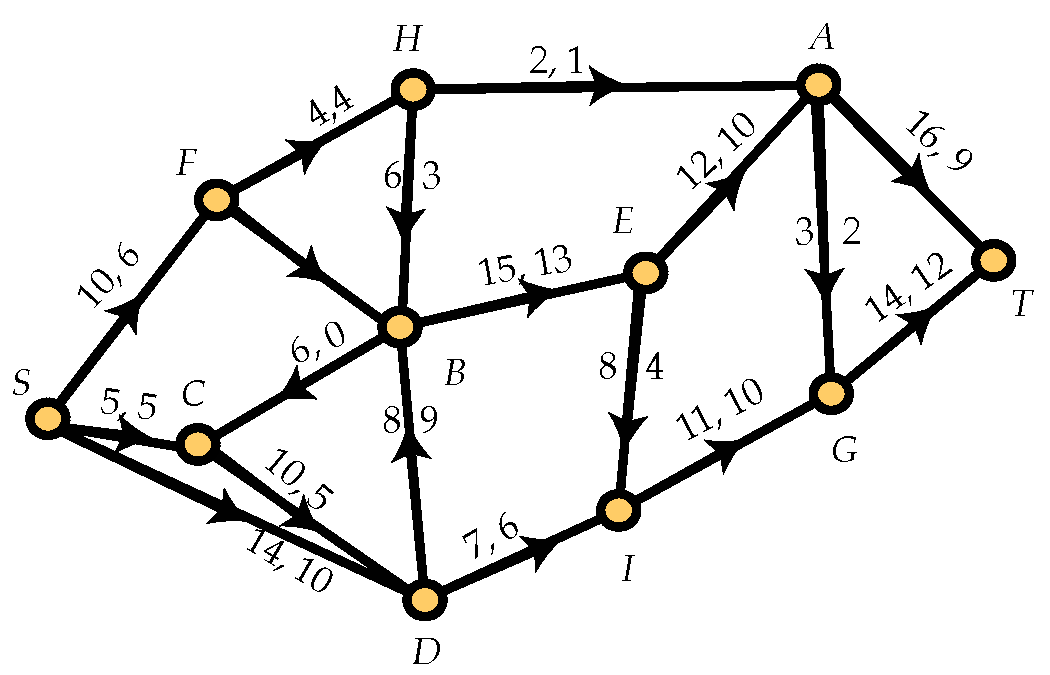
\includegraphics[width=3.5in]{networkflow-figs/networkflow_ex_invalid}
    \caption{An invalid flow in a network}
    \label{fig:networkflow:invalid}
  \end{figure}
\item Alice claims to have found a (valid) network flow of value $20$
  in the network shown in \autoref{fig:networkflow:network_ex}. Bob
  tells her that there's no way she's right, since no flow has value
  greater than $18$. Who's right and why?
  \begin{figure}
    \centering
    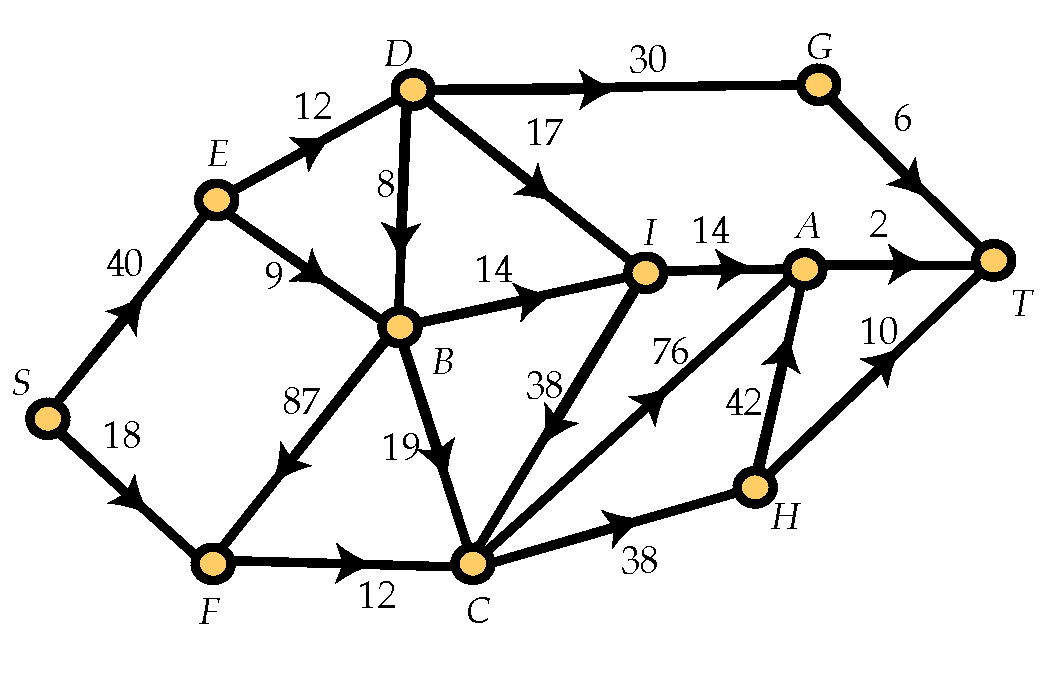
\includegraphics[width=3.5in]{networkflow-figs/network_ex}
    \caption{A network}
    \label{fig:networkflow:network_ex}
  \end{figure}
\item Find an augmenting path $P$ with \emph{at least one backward edge}
  for the flow $\phi$ in the network shown in
  \autoref{fig:networkflow:augpath_ex}. What is the value of $\delta$
  for $P$? Carry out an update of $\phi$ using $P$ to obtain a new
  flow $\hat{\phi}$. What is the value of $\hat{\phi}$?
  \begin{figure}
    \centering
    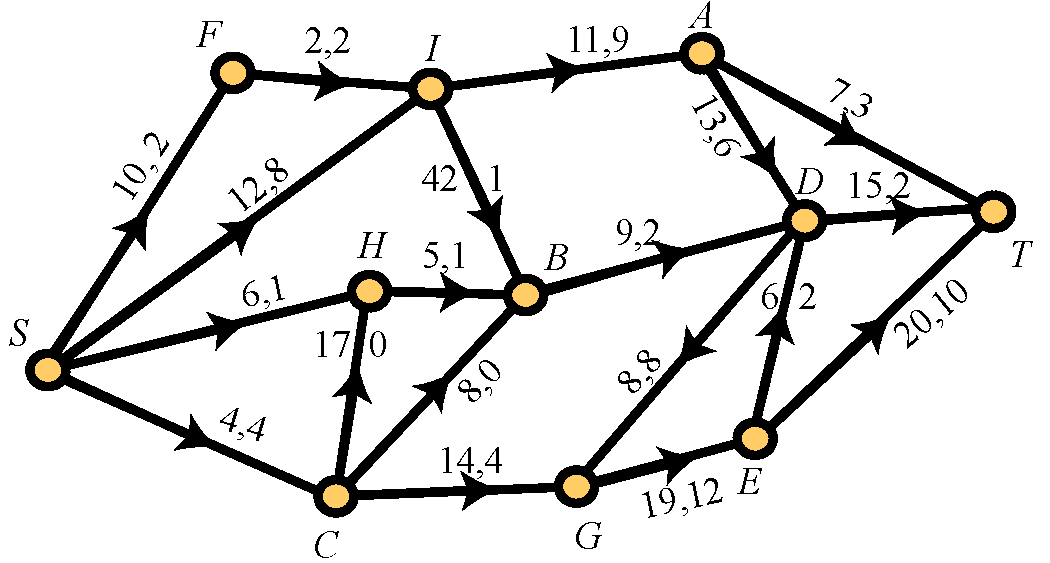
\includegraphics[width=3.5in]{networkflow-figs/augpath_ex}
    \caption{A network with flow}
    \label{fig:networkflow:augpath_ex}
  \end{figure}

\item Prove
  \hyperref[prop:networkflow:update]{Proposition~\ref*{prop:networkflow:update}}. You
  will need to verify that the flow conservation laws hold at each
  vertex along an augmenting path (other than $S$ and $T$). There are
  four cases to consider depending on the forward/backward status of
  the two edges on the augmenting path that are incident with the
  vertex.\label{ex:networkflow:update}
\item Find the capacity of the cut $(L,U)$ with
  \[L=\{S,F,H,C,B,G,I\}\qquad\text{and}\qquad U=\{A,D,E,T\}\]
  in the network shown in \autoref{fig:networkflow:augpath_ex}.
\item Find the capacity of the cut $(L,U)$ with
  \[L=\{S,F,D,B,A\}\qquad\text{and}\qquad U=\{H,C,I,G,E,T\}\]
  in the network shown in \autoref{fig:networkflow:augpath_ex}.
\item For each of the augmenting paths $P_1$, $P_2$, $P_3$, and $P_4$
  in
  \hyperref[exa:networkflow:delta]{Example~\ref*{exa:networkflow:delta}},
  update the flow in \autoref{fig:networkflow:netflow}. (Note that
  your solution to this exercise should consist of four network
  flows. Do not attempt to use the four paths in sequence to create
  one updated network flow.) \label{ex:networkflow:do-update}
\item Continue running the Ford-Fulkerson labeling algorithm on the
  network flow in \autoref{fig:networkflow:updated-flow} until the
  algorithm halts without labeling the sink. Find the value of the
  maximum flow as well as a cut of minimum capacity.
\item Use the Ford-Fulkerson labeling algorithm to find a maximum flow
  and a minimum cut in the network shown in
  \autoref{fig:networkflow:network_find_flow1} by starting from the
  current flow shown there.
  \begin{figure}
    \centering
    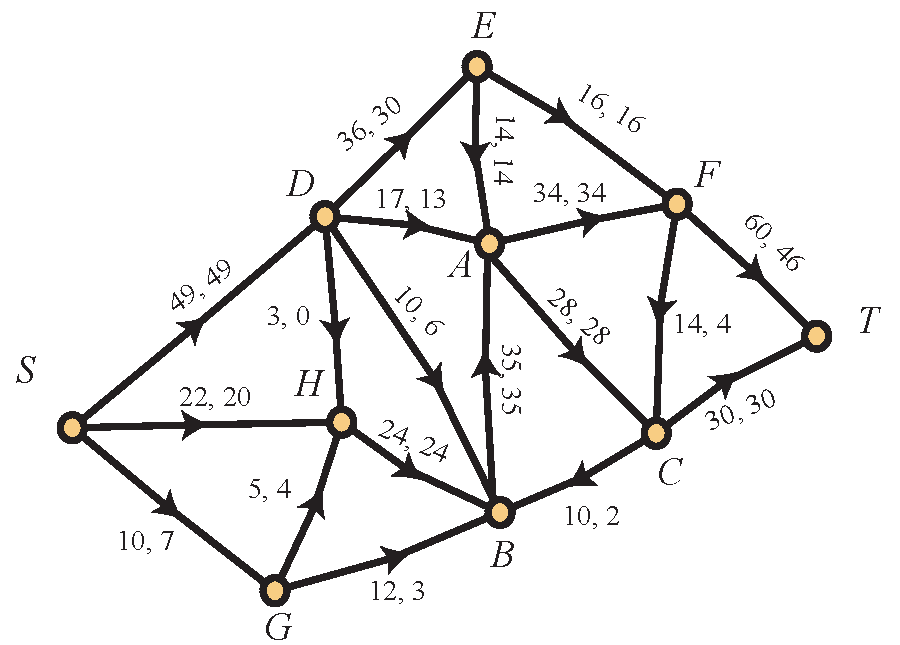
\includegraphics[width=3.5in]{networkflow-figs/network_find_flow1}
    \caption{A network with flow}
    \label{fig:networkflow:network_find_flow1}
  \end{figure}
\item \autoref{fig:networkflow:network_find_flow2} shows a
  network. Starting from the zero flow, i.e., the flow with
  $\phi(e)=0$ for every directed edge $e$ in the network, use the
  Ford-Fulkerson labeling algorithm to find a maximum flow and a
  minimum cut in this network.
  \begin{figure}
    \centering
    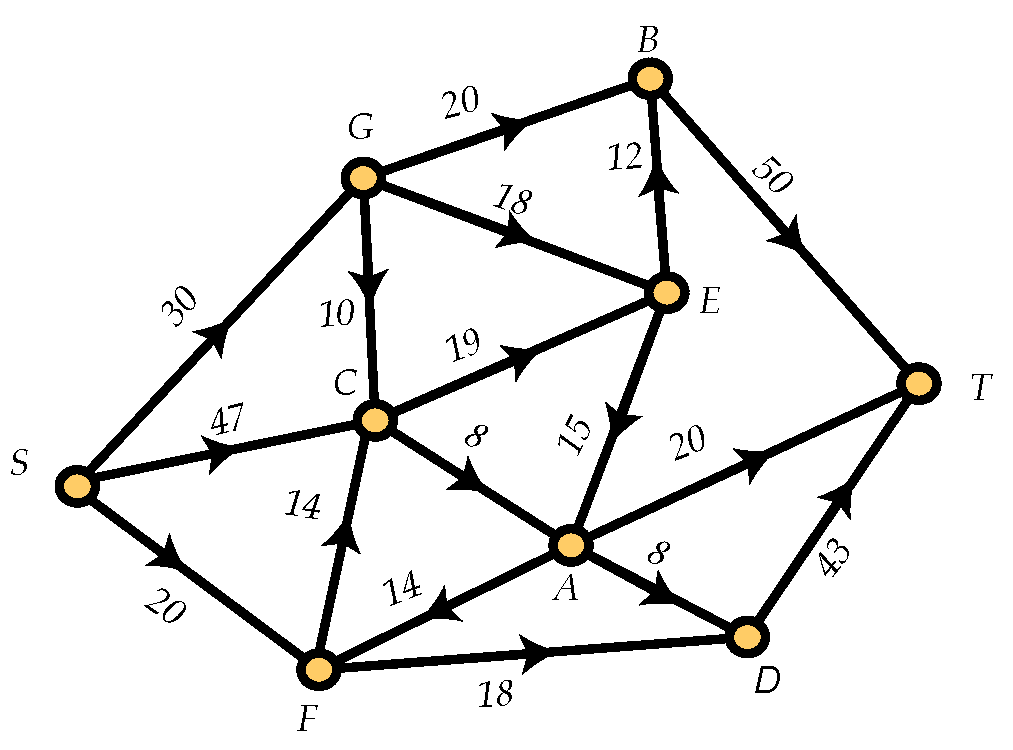
\includegraphics[width=3.5in]{networkflow-figs/network_find_flow2}
    \caption{A network}
    \label{fig:networkflow:network_find_flow2}
  \end{figure}
\item Consider a network in which the source $S$ has precisely three
  neighbors: $B$, $E$, and $F$. Suppose also that $c(S,B)=30$,
  $c(S,E)=20$, and $c(S,F)=25$. You know that there is a flow $\phi$
  on the network but you do not know how much flow is on any edge. You
  do know, however, that when the Ford-Fulkerson labeling algorithm is
  run on the network with current flow $\phi$, the first two vertices
  labeled are $S$ with label $(*,+,\infty)$ and $F$ with label
  $(S,+,15)$. Use this information to determine the value of the flow
  $\phi$ and explain how you do so.

\end{enumerate}

%%% Local Variables: 
%%% mode: latex
%%% TeX-master: "book"
%%% End: 
